\section{The modular tessellation and the exponential transformation}

In the theory of modular functions which we will touch in the next section, 
a map of essential importance is (in the notation of \Lehner{}) the transformation  $\ex : \C \to \C$, 
\begin{equation}
\ex(z) := \exp\left(2 \pi \ii z\right).
%\fundef{E}{\C}{\C}{z}{\exp(2 \pi \ii z).}
\end{equation}
Just like the Cayley transform, $\ex$ maps the upper half-plane onto the unit disk $\mathbb{D}$, as we see through
\begin{equation*}
\abs{\ex(z)} = 
\exp\left(\Re{2 \pi \ii z}\right) = 
\exp\left(-2 \pi \Im{z}\right).
\end{equation*}
Obviously $\Im{z} > 0$ implies $\abs{\ex(z)} < 1$ and the real axis is mapped to the boundary of $\mathbb{D}$. In contrast to the Cayley transform, $e$ is not a one-to-one map from the upper half-plane to the unit disk, as clearly $e(z) = e(z + k)$ for arbitrary $k \in \Z$. Instead it can be considered as a bijective map from the strip 
\begin{equation*}
S = \setdefsz{\big}{z \in \C}{\Re{z} \in \left[-0.5,0.5\right),\ \Im{z} \ge 0}
\end{equation*}
to the punctured unit disk $\mathbb{D} \setminus \{0\}$. Note that the exponential function has an essential singularity at the point $\infty$, but still it is sometimes useful to define $e(\infty) := 0$. This is motivated by a continuous extension of $e$ from the domain $S$ to $S_\infty := S \cup \{\infty\}$ by
\begin{equation*}
e(\infty) := \lim_{\substack{\Im{z} \to \infty\\z \in S}} e(z) = 0.
\end{equation*}
In this way we obtain a bijective map from $S_\infty$ to the closed unit disk $\mathbb{D}$. We now can use $e : S_\infty \to \mathbb{D}$ to map the modular tessellation of the upper half-plane -- to be precise, the part of it which lies within $S_\infty$ -- to the unit disk. The result can be seen in Figure~\ref{fig_ModularTilingExp}.

\begin{figure}
\centering
\includegraphics[width=\textwidth]{figures/modular-tiling-exp}
\caption{The modular tessellation under the transformation $z \mapsto e(z)$. The equation $\abs{z} = \exp(-2\pi \ii \Im{z})$ implies that points with large imaginary part are mapped very closely to $0$. In particular the image of the fundamental domain $\FunDom$ cannot be seen in this scale any more. Its points, satisfying $\Im{z} > \frac{\sqrt{3}}{2}$, are mapped into a disk centered about the origin of a radius smaller than $0.005$.}
\label{fig_ModularTilingExp}
\end{figure}

For a better understanding on how $S_\infty$ is deformed to the unit disk by the transformation $\ex$, we can again take advantage of a simple M�bius transformation: The map
\begin{equation*}
f(z) := \frac{\ii}{z + \\i}
\end{equation*}
maps the upper half-plane to a disk of radius $1/2$ centered about the real point $1/2$. The choice of $f$ is not as arbitrary as it seems, because
\begin{equation*}
f(0) = \ex(0) = 1 \quad\text{and}\quad f(\infty) = \ex(\infty) = 0.
\end{equation*}
In Figure~\ref{fig_ModularTilingExpFan} we can see a continuous transition from the images of the modular tessellation on $S_\infty$ under the M�bius transformation $f$ and the respective image under $\ex$. The shape of $f(S_\infty)$ is bounded by three circular arcs, as we can see in the first (top-left) frame of Figure~\ref{fig_ModularTilingExpFan}. It is continuously fanned out to whole unit disk through the map
\begin{equation*}
h(t, z) := f(z)^{1-t} \cdot e(tz).
\end{equation*}

\begin{figure}
\centering
\includegraphics[width=\textwidth]{figures/modular-tiling-exp-fan}
\caption{The tessellation under the transformation $z \mapsto \exp(2 \pi \ii z)$.}
\label{fig_ModularTilingExpFan}
\end{figure}

\begin{figure}
\centering
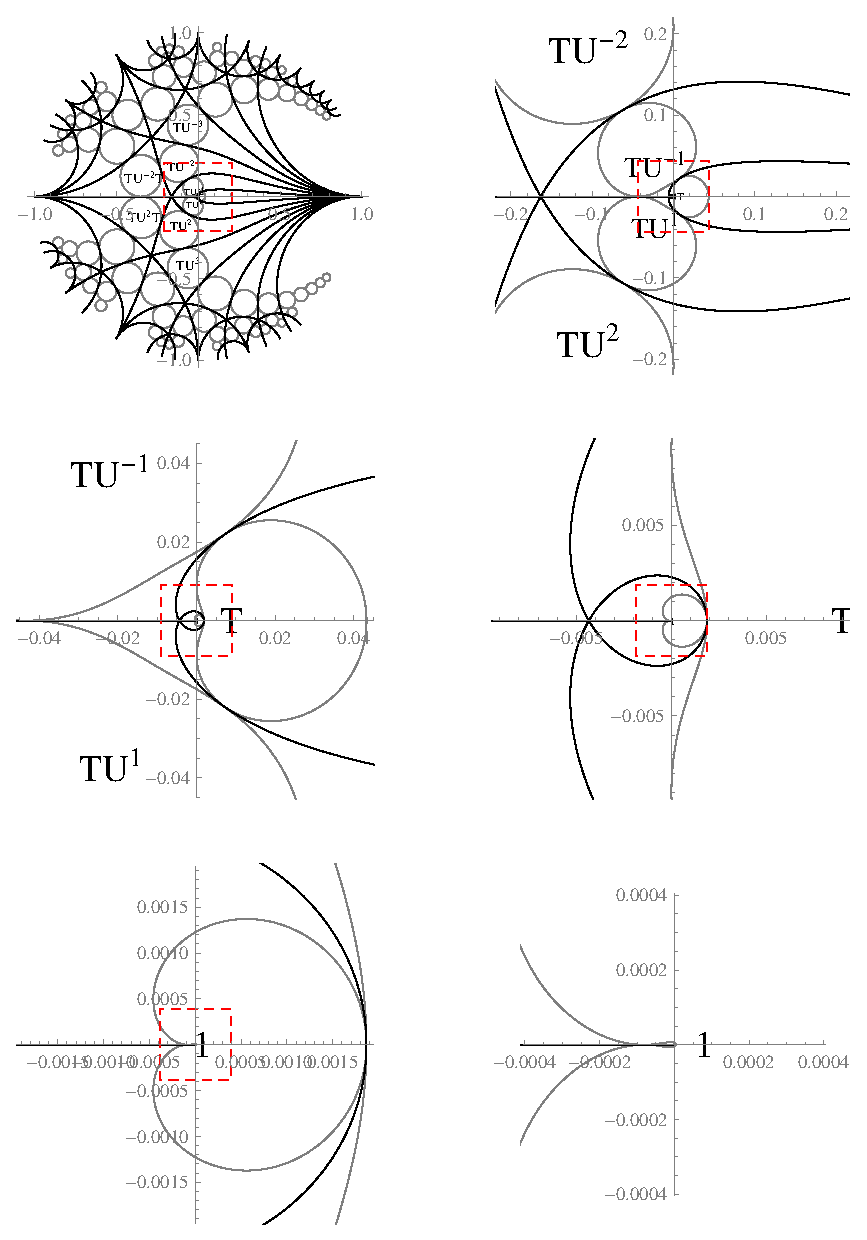
\includegraphics[width=\textwidth]{figures/modular-tiling-exp-zoom}
\caption{The image of the modular tiling under the map $z \mapsto \exp(2 \pi \ii z)$ in the neighborhood of $\infty$.}
\label{fig_ModularTilingExpZoom}
\end{figure}
